\documentclass[12pt, twoside]{article}
\input{/Users/chris/github/course-files/docs/ib/preamble}

\fancyhead[LE]{\thepage}
\fancyhead[RO]{Name: \hspace{4cm} \,\\ \hspace{2.9cm} \,}
\fancyhead[LO]{La Scuola d'Italia / Dr.\ Huson / IB Math 12 HL \\* 9 September 2026}

\begin{document}
\subsubsection*{12.3 Classwork: Complex Numbers: Polar Form and de Moivre (no calculator)}

Answer both problems in the spaces provided. Show your working. Give
all answers as exact values (surds and fractions of $\pi$), not decimals.

\begin{enumerate}[itemsep=0.15cm]

%--- Problem 1: Cartesian arithmetic, modulus, real unknowns [7 marks] ---
%--- Source: authored 2026-09-07 (HL syllabus 1.12) ---

%--- Problem 3: Modulus-argument and exponential form, Argand plot [8 marks] ---
%--- Source: authored 2026-09-07 (HL syllabus 1.13) ---
\item[1.]

Consider the complex numbers $z = -1 + i\sqrt{3}$ and $w = 2 - 2i$.

In parts (a) to (c), give every argument $\theta$ in the range
$-\pi < \theta \leq \pi$.

\begin{enumerate}[itemsep=0.15cm]
  \item Write $z$ in the form $r(\cos\theta + i\sin\theta)$ and in the form
  $re^{i\theta}$.
  \item Write $w$ in the form $r(\cos\theta + i\sin\theta)$ and in the form
  $re^{i\theta}$.
  \item Hence find $zw$ and $\dfrac{z}{w}$, giving each answer in the form
  $re^{i\theta}$.
  \item On the Argand diagram below, plot and label the points representing
  $z$, $w$ and $zw$.
\end{enumerate}

\begin{center}
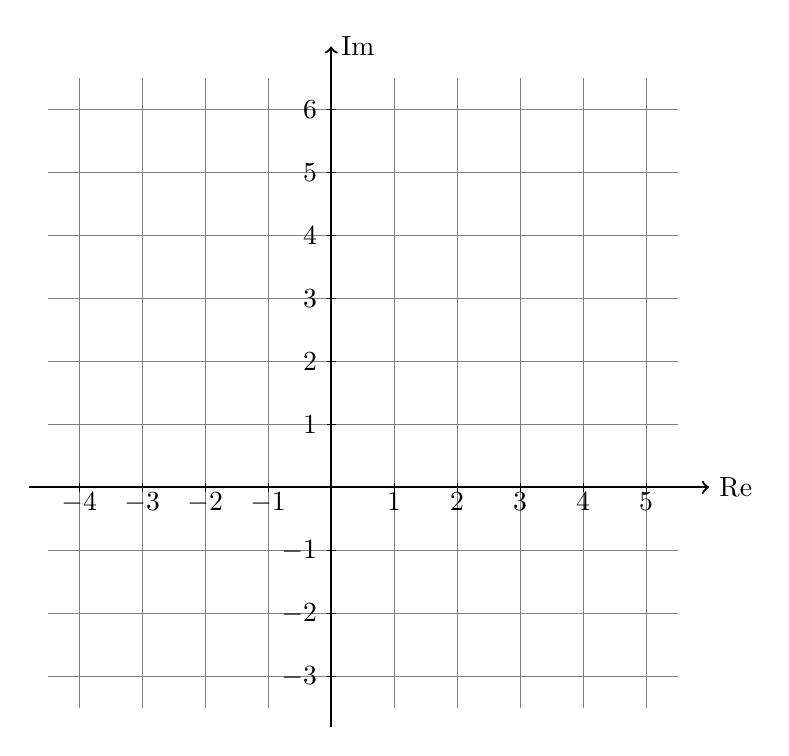
\begin{tikzpicture}[scale=0.8]
  \draw [thin, color=gray, xstep=1.0cm, ystep=1.0cm] (-4.5,-3.5) grid (5.5,6.5);
  \foreach \x in {-4,-3,-2,-1,1,2,3,4,5}
    \draw[shift={(\x,0)}, color=black] (0pt,-2pt) -- (0pt,2pt) node[below] {$\x$};
  \foreach \y in {-3,-2,-1,1,2,3,4,5,6}
    \draw[shift={(0,\y)}, color=black] (2pt,0pt) -- (-2pt,0pt) node[left] {$\y$};
  \draw [thick, ->] (-4.8,0) -- (6.0,0) node [right] {$\mathrm{Re}$};
  \draw [thick, ->] (0,-3.8) -- (0,7.0) node [right] {$\mathrm{Im}$};
\end{tikzpicture}
\end{center}

\begin{tikzpicture}
  \draw (-0.6,0) rectangle (11,5);
  \foreach \y in {1,2,...,4} \draw[dotted] (0,\y)--(10.5,\y);
\end{tikzpicture}

\newpage

%--- Problem 4: de Moivre's theorem, cube roots of 8i [7 marks] ---
%--- Source: authored 2026-09-07 (HL syllabus 1.14) ---
\item[2.]

\begin{enumerate}[itemsep=0.15cm]
  \item Use de Moivre's theorem to find the exact value of $(1 + i)^8$.

  \item Find the three cube roots of $8i$, giving each answer in the form
  $re^{i\theta}$, where $r > 0$ and $-\pi < \theta \leq \pi$.
  \item State the geometric relationship between the three cube roots of
  $8i$ when they are plotted on an Argand diagram.
\end{enumerate}

\begin{tikzpicture}
  \draw (-0.6,0) rectangle (11,16.5);
  \foreach \y in {1,2,...,15} \draw[dotted] (0,\y)--(10.5,\y);
\end{tikzpicture}

\end{enumerate}
\end{document}